\chapter{Implementation Details}\label{chap:implementation_details}
This chapter discusses the implementation details of the developed project referencing technologies used throughout the development process, the code architecture and other implementation specific information related to the project. 

\section{Chewie}
During the course of the project, I have worked towards developing Chewie; an 802.1x Authenticator written in Python3. \\
Chewie is written to function as a stand-alone application for processing 802.1x requests, but is primarily intended for use with the Faucet SDN controller.\\
Chewie's design philosophy is an extension to Faucet's; aiming for easily-legible code using small and reusable code segments in an attempt to provide a light-weight solution for network authentication.
The architecture focuses primarily on leveraging functionality present in 802.1x applications, acting exclusively as an Authenticator; translating EAPoL to RADIUS and forwarding messages.

As ingress packets arrive through the supplicant-facing interface, they are translated into their respective RADIUS equivalents and forwarded through a RADIUS-facing interface for processing. This allows the RADIUS server to perform all identity and authentication checks whilst allowing Chewie to be aware of all changes in authentication state.

State is maintained in Chewie through the use of state machines, allowing for detection of any deviation from the expected packet-flow, such as attempting to bypass the authentication by starting communications with an authentication successful response.

On a successful authentication event, Chewie notifies Faucet of the authentication status change through a custom plugin API. Client information and session restrictions are sent with notification messages allowing Faucet to add restrictions on client sessions. 
Likewise, Chewie is notified of any changes of state for managed ports through the same interface.

This custom Chewie/Faucet API required small amounts of additional code to be added to the main Faucet code-base, which has now been merged into the main open-source project\cite{faucet_github}. The current version of Faucet (Version 1.5.9) has full Chewie support. 

The Chewie code is provided as a separate repository\cite{chewie_github} which is also open-source.

\section{Functionality Overview}
Chewie's functionality can be split into 4 major components listed below and explained in further detail in the following sections.

\begin{enumerate}
    \item RADIUS communication
    
    All communication between Chewie and the RADIUS server is achieved through the use of a datagram socket. Using a network connection separate to the data network, Chewie and RADIUS are able to send messages using UDP, as per the RADIUS specification. \cite{radius_why_udp}
    
    \item Faucet communication
    
    Communication between Faucet and Chewie is achieved through a custom API written into Faucet. This API uses callback functions to notify Faucet of authentication events as they occur. Chewie is also notified on port-up and port-down events through function calls. \cite{faucet_dot1x_docs}

    \item Supplicant communication
    
    Communication between Chewie and the connecting Supplicant is achieved through the use of an NFV port connected to the data network. Faucet forwards relevant traffic originating from managed ports to the closest NFV port where it is consumed by one of two  listening sockets. One socket is dedicated to receiving EAPoL requests and the other dedicated to receiving DHCP requests.
    
    \item State Management
    Authentication state in Chewie is managed through the use of state machines. When a request arrives from a new client, a new state-machine is generated and attached to the authenticating client. The state machine is then used to manage the authentication process for that client. There are two types of state machine in Chewie, an EAP state machine used for managing the EAP authentication process and a MAB state machine used for performing MAB authentication.
\end{enumerate}

\section{Faucet Communication}
\subsection{Authentication Events}
In Python3, functions are handled as first-class objects. This allows them to be stored and passed around like variables. Communication between Faucet and Chewie leverages this functionality, passing callback functions to Chewie on instantiation. These callback functions are used to notify Faucet of authentication events as they occur.\\
Definitions for the callback functions have been provided below, explaining expected parameter values and expected Faucet behaviour.
\begin{itemize}
    \item \textbf{auth\_handler}\\
    This callback function is used to notify Faucet of a successful authentication. The function requires information about the client, including the MAC address, port location and any restrictions to be placed on the session such as a VLAN identifier and/or ACLs to be applied to the session. It is expected that this function will apply all relevant restrictions and open the provided port for communication with the secure network.
    
    \item \textbf{logoff\_handler}\\
    This callback function is used to notify Faucet of a successful logoff event. The function requires information about the client, including the MAC address and port location. It is expected that this function remove the authenticated session for the given MAC address on the provided port. The client will no longer have the ability to communicate with the secure network.
    
    \item \textbf{failure\_handler}\\
    This callback function is used to notify Faucet of an unsuccessful authentication attempt. The function requires information about the client, including the MAC address and port location. It is expected that this function remove an authenticated session for the given MAC address on the provided port, if present. The client will not have the ability to communicate with the secure network after the completion of this handler.
\end{itemize}

\subsection{Port Status Events}
On instantiation, Faucet retains a copy of the Chewie object and uses it to notify Chewie of any state changes of managed ports. This is done through calling methods provided by the Chewie public interface. The relevant methods are defined below, defining the expected parameter values and expected Chewie behaviour.
\begin{itemize}
    \item \textbf{port\_up}\\
        Triggered in the event of a port-up event, Faucet builds and deploys flows to direct all EAPoL traffic to the closest NFV port. If MAB is active on the port then DHCP traffic is also forwarded. Chewie is notified of the change in status and must start sending pre-emptive identity requests looking for clients to authenticate.
    \item \textbf{port\_down}\\
        Triggered in the event of a port-down event. Faucet destroys all flows for the port, removing any VLANs and ACLs associated with the port. Chewie is notified of the change in status, must stop any outstanding jobs and destroy all objects associated with the port.
\end{itemize}

In future development it is proposed that the callback system be removed and replaced with Google's Remote Procedure Call functionality, gRPC\cite{grpc_website}. This will allow for better separation of concerns, creating a clear barrier between Chewie and Faucet and allow Chewie to scale without the need for Faucet. It will also allow Chewie to connect to SDN controllers that are not written in Python. [For further reading; Refer to Chapter \ref{chap:future_development}]

\section{RADIUS Communication}
RADIUS communication is achieved through a RADIUS-facing interface separate from the data network. It has been separated to stop any clients attempting to communicate directly with the RADIUS server. 
Chewie provides options for all standard RADIUS packet-types for authentication. These include Access-Request, Access-Challenge, Access-Accept and Access-Reject packets which are defined in Section \ref{sec:radius_packets}.\\
RADIUS Accounting \cite{radius_accounting} is not provided by mainline Chewie but is available in an experimental branch. \cite{chewie_radius_accounting}\\

\section{Supplicant Communication}
Communication with the connecting client is achieved through a 2-step process.
\subsection{EAPoL}
First, as the client connects to a managed port, Faucet deploys flows to route all EAPoL traffic to the closest NFV port.\\
Secondly, as frames are received by the switch they are marked with their origin. As no extra information can be attached to an EAPoL frame without introducing another protocol layer, the origin port and switch of the frame is marked in-place of the destination MAC address (DST MAC) and the frame is forwarded to the NFV port using flow actions.
The origin marking consists of a 2-byte number representing the switch index in the local network and the port number within the switch. These numbers are padded with 0's to meet the required 48-bits for the DST MAC field.

As the DST MAC field is not that of Chewie's supplicant-facing NIC, the supplicant-facing socket must be placed into promiscuous mode for Chewie to receive the expected traffic.

Once the socket receives a frame, the origin is extracted from the DST MAC and recorded against the frame for future reference and the EAPoL frame is sent to the EAP state machines for processing.

\subsection{MAB}
If MAB is active on the port, DHCP traffic is also forwarded to the NFV port with the EAPoL traffic, the ETH DST value is overwritten and the DHCP packets are forwarded to the supplicant-facing interface using flow rules.

Once the MAB socket receives a DHCP packet, the origin is extracted from the DST MAC and recorded against the frame for future reference and the DHCP packet is sent to the MAB state machines for processing.

\section{Managing Authentication State}
The current authentication status of clients is maintained through a list of state machines (SM). As a new client attempts to authenticate, a state machine unique to their origin port and MAC address is created. This state machine follows the authentication process and ensure that there is no deviation from the expected packet-types. The state machines also regulate which requests may be forwarded through to the RADIUS server.

There are two types of state machines that are used to process user authentication; The MAB state machine (MAB SM), which is used to perform all MAB requests and the EAP state machine, which is used to process all EAPoL authentication requests.

\subsection{MAB State Machine}
\begin{figure}\begin{center}
    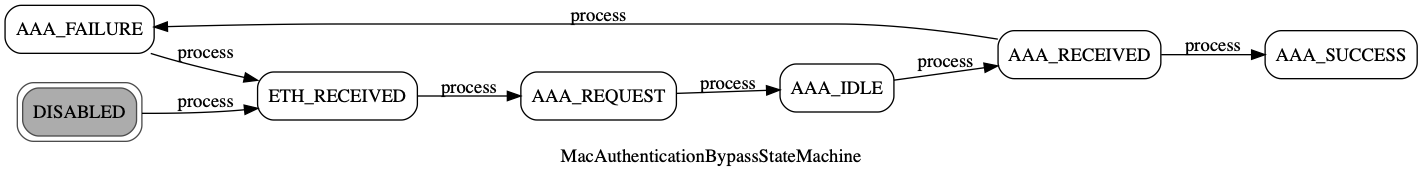
\includegraphics[height=1.5cm]{images/mab_state_machine.png}
    \caption{MAB State Machine}
    \label{fig:mab_state_machine}
\end{center}\end{figure}

As a DHCP request is received on the NFV port, a MAB state machine is created and passed the DHCP request. The MAB state machine uses the DHCP request to generate a RADIUS Access-Request containing the MAC address of the client as the following attributes:
\begin{itemize}
    \item \textbf{IETF 1 - User-Name} 
    
    Stored in plain text with no separators
    \item \textbf{IETF 2 - User-Password} 
    
    Stored as ciphertext. All separators are removed and the MAC address is encrypted using the MD5-based algorithm defined in the RADIUS RFC\cite{radius_password_attribute}
    \item \textbf{IETF 31 - Calling-Station-ID} 
    
    Stored in plain text, separating digit-pairs using a hyphen ('-')
\end{itemize}

On receiving the request, the state machine transitions from the 'DISABLED' state into the 'ETH\_RECEIVED' state for processing. The MAC address is extracted from the packet and store in the SM. A RADIUS request is generated according to the above attributes and send to the RADIUS server, transitioning the SM through the 'AAA\_REQUEST' state to the 'AAA\_IDLE' state, where it waits for a response from the RADIUS server.

On receiving a response from the RADIUS server, the state transitions to 'AAA\_RECEIVED'. 

If the response is successful the SM transitions to 'AAA\_SUCCESS' and the 'auth\_handler' callback function is triggered opening the session. 

Likewise, if the response is unsuccessful the SM transitions to 'AAA\_FAILURE' and the 'failure\_handler' is triggered, forcing the session closed.

For more information about state transitions, refer to Figure \ref{fig:mab_state_machine}.

\subsection{EAP State Machine}
\begin{figure}\begin{center}
    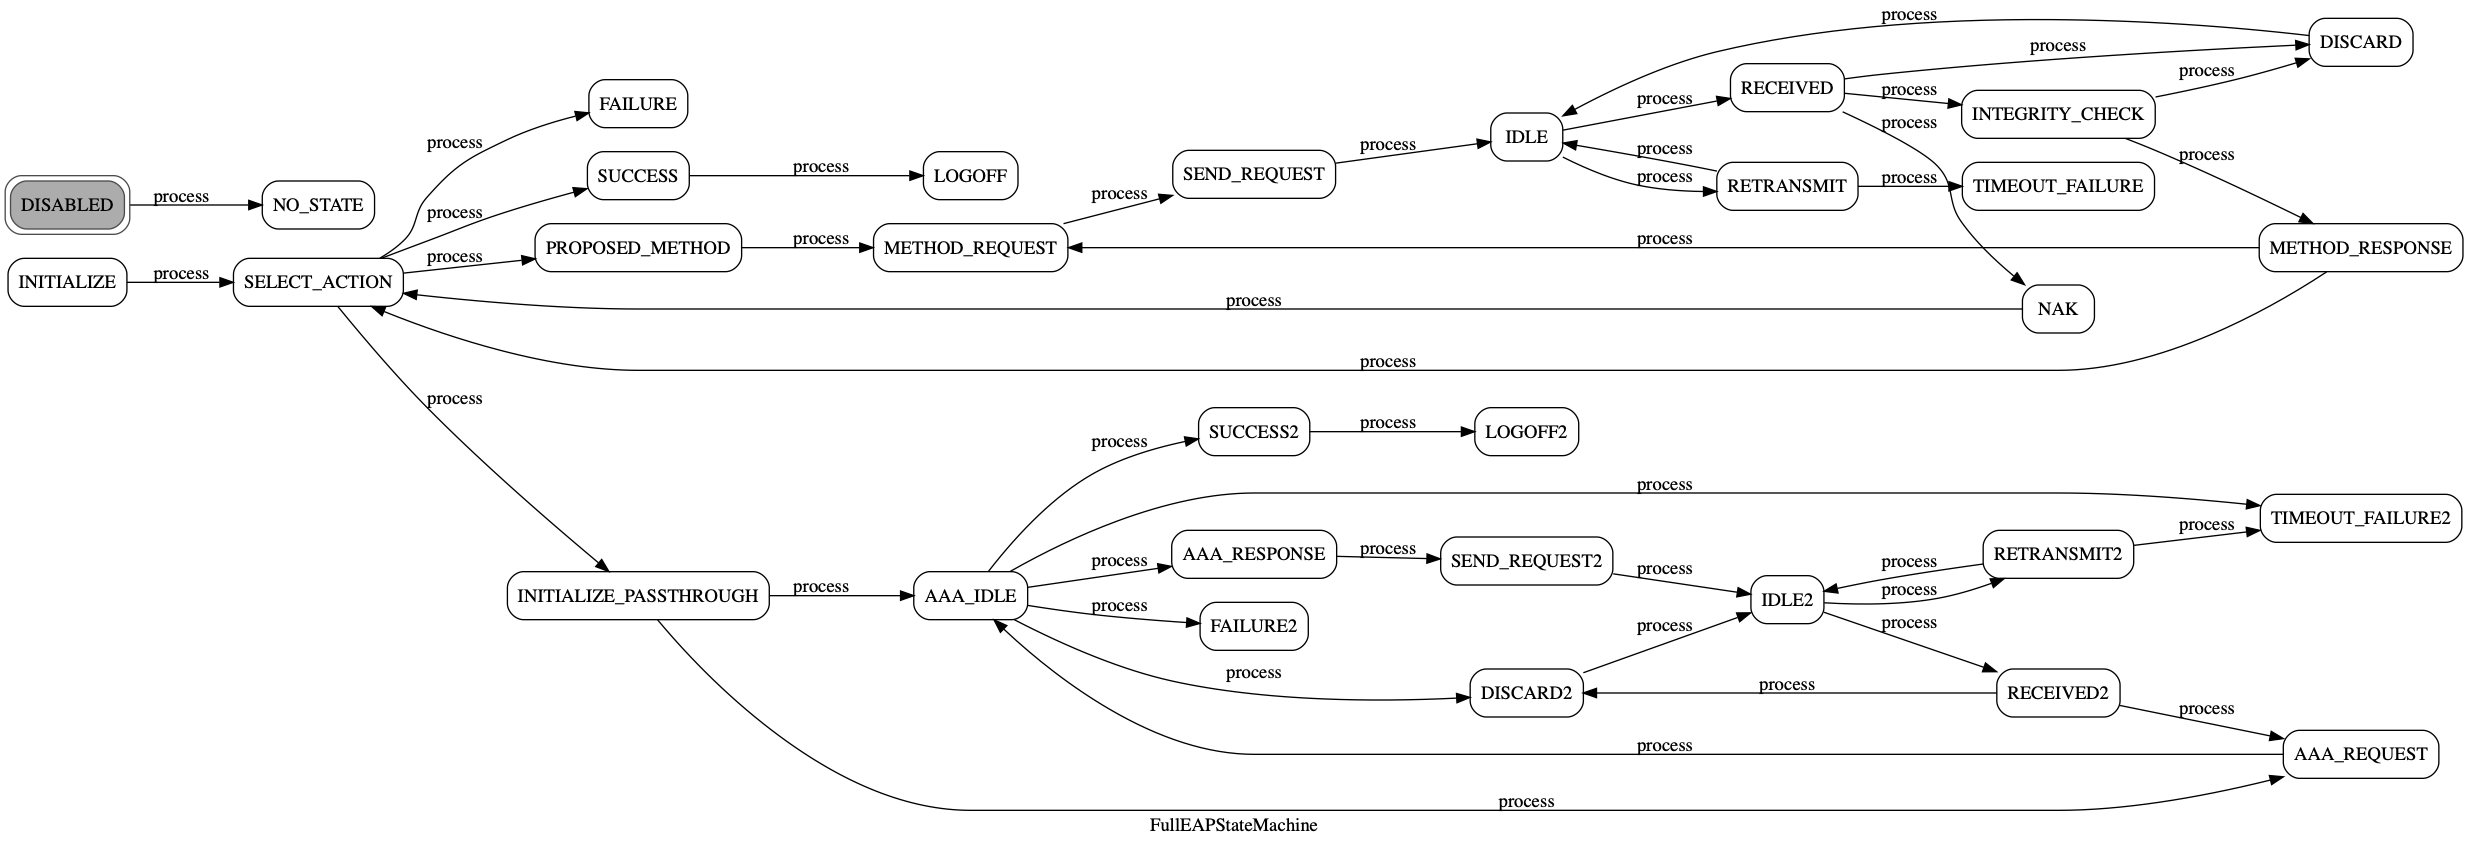
\includegraphics[height=4.7cm]{images/eap_state_machine.png}
    \caption{EAP State Machine}
    \label{fig:eap_state_machine}
\end{center}\end{figure}

The state machine defined in RFC 4137\cite{rfc_4137} is used as the basis of the EAP state machine (EAP SM) implementation. Initially deviating from the defined state machine through the introduction of the 'LOGOFF' and 'LOGOFF2' states, we have extended upon the original state machine design for increased code clarity and reuse.
Our EAP SM implementation can be split into 3 functional segments listed below:
\begin{itemize}
    \item \textbf{Method Negotiation}
    
    Method negotiation is performed to ensure that both parties communicate using the same EAP method.\cite{rfc_3748}. Chewie notifies the Supplicant that EAP pass-through is required and all following authentication requirements are performed by the authentication server.
    
    \item \textbf{Local Authentication}
    
    Local authentication is provided by the EAP state machine in accordance with RFC 4137\cite{rfc_4137} but is not implemented nor supported.
    
    \item \textbf{RADIUS Authentication}
    
    RADIUS authentication is the intended verification technique and involves the Supplicant performing an authentication process with the RADIUS server. All EAP-based RADIUS authentication methods supported by Chewie require a challenge to be performed by the Supplicant. The challenge is performed in accordance with the EAP method chosen and provided back to the RADIUS server to prove identity.
\end{itemize}

As a request is received by the EAP state machine, the SM transitions to the 'SELECT\_ACTION' state, where the 'Method Negotiation' segment is initiated. The available EAP authentication methods are proposed by Chewie to the supplicant and an EAP method is agreed upon.
On successful completion of 'Method Negotiation', the SM is returned to the 'SELECT\_ACTION' state to initiate the second phase of authentication.

If the outcome is 'Local Authentication', the SM is transitioned into either the 'SUCCESS' or 'FAILURE' state depending on the result of a local look-up for the provided credentials. If the credentials provided successful authentication the SM transitions to the 'SUCCESS' state and 'auth\_handler' is called, if the credentials fail to provide a success authentication the SM transitions to the 'FAILURE' state and the 'failure\_handler` is called.

If the outcome is RADIUS authentication, the SM is transitions into the 'INITIALIZE\_PASSTHROUGH' state and the RADIUS authentication process begins.

RADIUS authentication is discussed further in the following section as it pertains to both the EAP State Machine and the MAB State Machine. For further information about the EAP SM state transitions, refer to Figure: \ref{fig:eap_state_machine}.

\section{RADIUS Authentication}
Successful RADIUS authentication can be achieved through providing user-credentials in the initiating RADIUS Access-Request packet, using RADIUS attributes. This method is used by Chewie's MAB implementation.

EAP authentication is achieved through the result of a generated challenge provided to the Supplicant. The result of the challenge is provided back to the RADIUS server where it is used to complete the authentication process.

Both authentication methods are initiated using a RADIUS Access-Request sent from Chewie to the RADIUS server.

\subsection{AAA Authentication}
The MAB state machine performs RADIUS authentication providing required information as RADIUS attributes. On receiving the first RADIUS Access-Request, the RADIUS server is provided with enough information to verify a clients identity and provide an authentication response. For MAB this is achieved through the use of the User-Name and User-Password attributes and is the authentication-type used for MAB implementation in Chewie. For further information on the packet flow required for challenge-free authentication refer to \ref{fig:no_challenge_radius}
\begin{figure}\begin{center}
    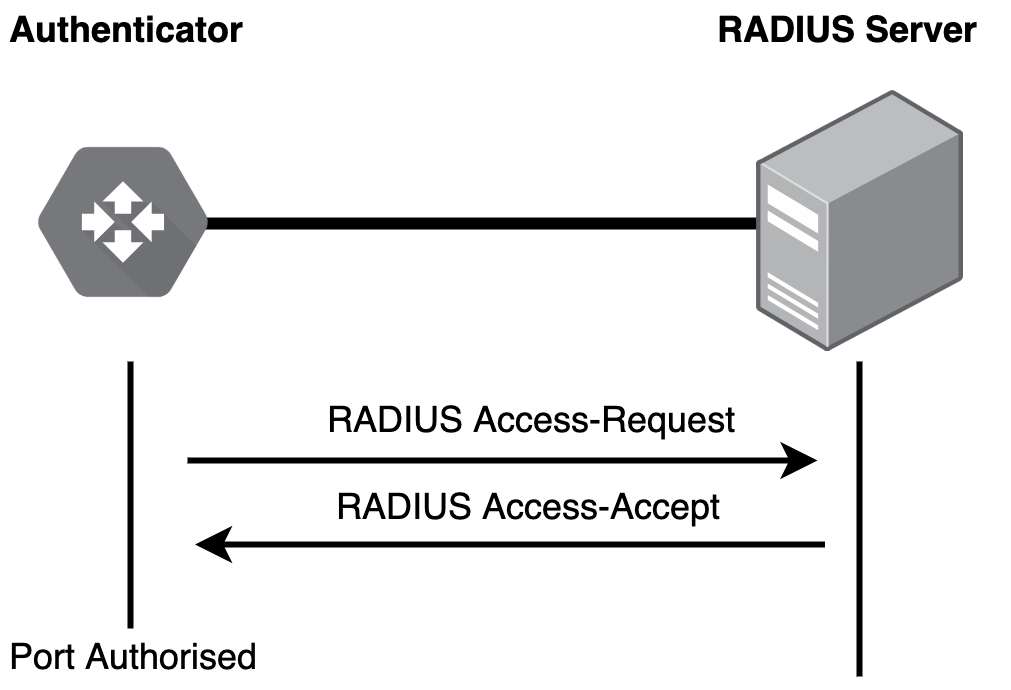
\includegraphics[height=4cm]{images/no_challenge_radius.png}
    \caption{Challenge-Free RADIUS Packet Flow}
    \label{fig:no_challenge_radius}
\end{center}\end{figure}

\subsection{EAP Authentication}
Challenged authentication is required to perform an EAP-based authentication. Once the EAP-method negotiation has completed, an EAP Identity Response is sent from the Supplicant. The Authenticator (Chewie) encapsulates the EAP Response in a RADIUS Access-Request packet and forwards the request to the RADIUS server for processing.

On receiving the RADIUS encapsulated EAP packet, an EAP-challenge is generated and sent back to the Supplicant. The challenge is performed in accordance with the selected EAP method and the result is sent to the RADIUS server completing the EAP authentication process. A RADIUS Access-Accept or RADIUS Access-Reject is then provided, if the authentication is successful or unsuccessful respectively. For further information on the packet flow for challenged authentication, refer to \ref{fig:challenge_radius}
\begin{figure}\begin{center}
    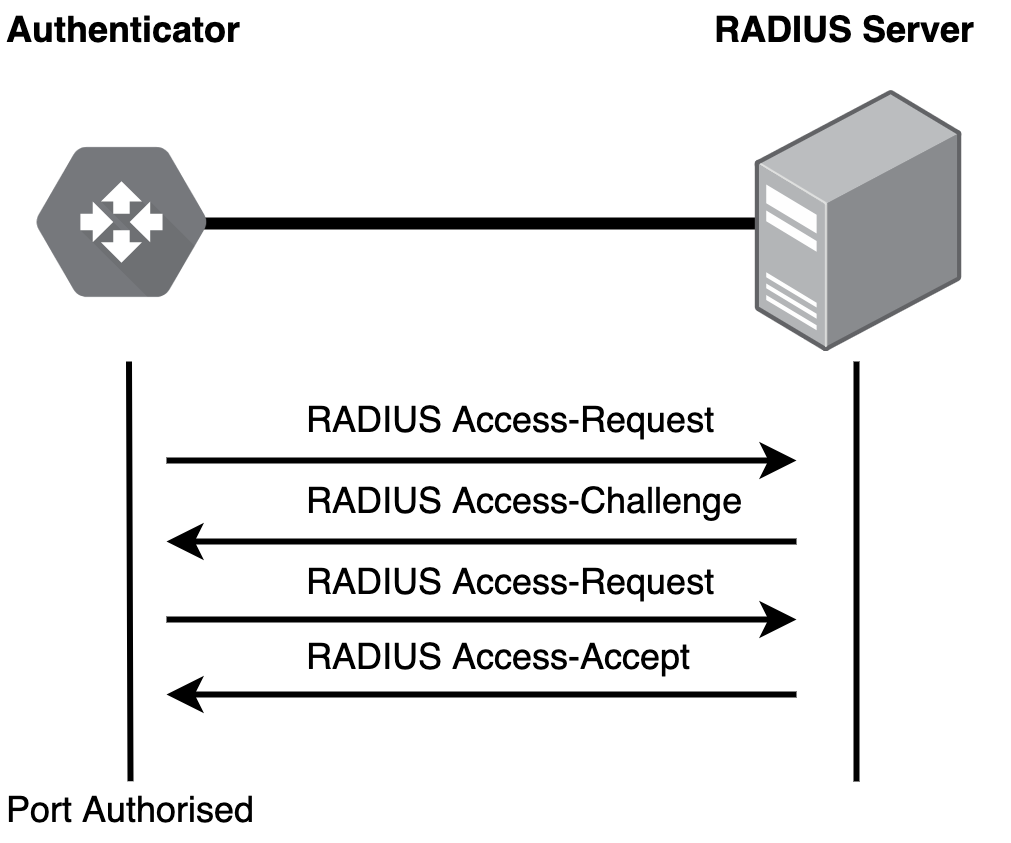
\includegraphics[height=5cm]{images/challenge_radius.png}
    \caption{EAP Challenge RADIUS Packet Flow}
    \label{fig:challenge_radius}
\end{center}\end{figure}


\section{Configuration}
Faucet is configured through the use of a YAML file. Configuration is read by Faucet and passed to Chewie on start-up. For a port to be controlled by Chewie, it must be marked as a 802.1x port in the Faucet configuration file.
Along with controlled ports, the configuration file contains values for connecting with the RADIUS server. These values include authentication credentials, the RADIUS server IP address, RADIUS-facing interface, the Supplicant-facing interface and NFV port locations.
All related preferences are provided to Chewie as arguments during initialisation.

Once a port is marked as a controlled port, flow rules are deployed for forwarding EAPoL traffic to the NFV port.

NFV ports are defined in the Faucet configuration file, defining the port number and switch id that Chewie is connected to on the data-network. All authentication requests from managed ports are routed to the NFV port for processing. \cite{faucet_dot1x_docs}

\section{Applying Session Restrictions (RBAC)}
On successful authentication, the RADIUS server notifies Chewie using a RADIUS Access-Accept packet, attaching any VLAN and RBAC session requirements as RADIUS attributes. 
If present, Chewie passes these requirements to Faucet with an authentication status change event. Faucet builds all flow rules in accordance with the provided restrictions and distributes flows to relevant switches.

VLAN requirements are passed to Chewie using the Tunnel-Type (IETF 64), Tunnel-Medium-Type (IETF 65) and Tunnel-Private-Group-ID (IETF 81) RADIUS attributes.

RBAC requirements are passed to Chewie by defining the ID of an ACL to be applied on the authenticated port. The attribute used for transporting the ACL ID is Filter-Id (IETF 11).\cite{faucet_dot1x_docs}

All used ACLs must be known by Faucet on startup and defined in the Faucet configuration file. This is required as Faucet allocates matching resources on switches at start-up and must be restarted to defined new matching fields.